\documentclass[a4paper,17pt]{extarticle}
\usepackage[utf8]{inputenc}
\usepackage{amsmath}
\usepackage{amssymb}
\usepackage{fontspec}
\usepackage[T1]{fontenc}
\usepackage{caption}
\usepackage{hyperref}
\usepackage{array}
\usepackage{tabularx}
\usepackage{graphicx}
\usepackage{background} 
\usepackage{float}
\backgroundsetup{contents=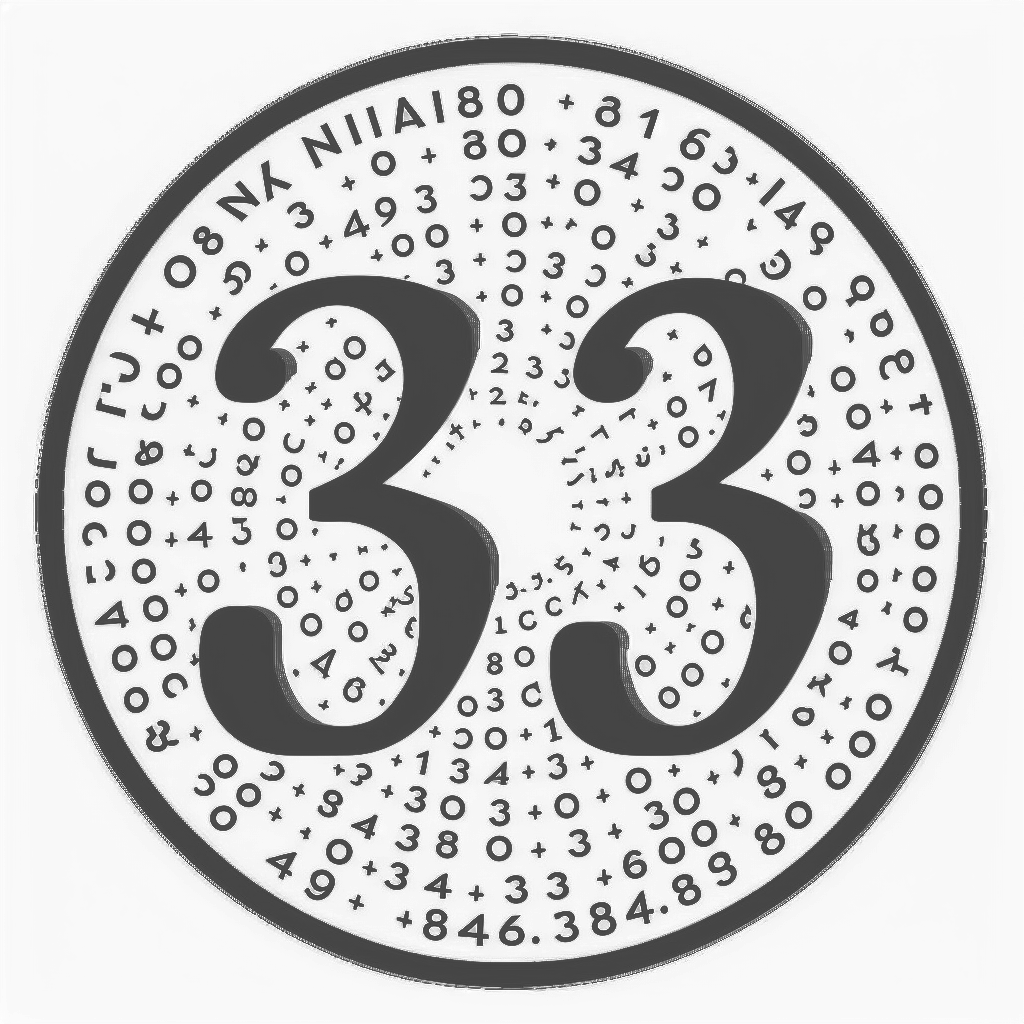
\includegraphics{static/logo.png}, opacity=0.1, scale=.3, angle=0}
\title{Inverse Pythagorean Theorem}
\author{Saugat Dhakal, Asal KC }
\date{February 2023}

\begin{document}

\maketitle

\section{}
\textbf{Problem:} Prove that in a right angles triangle, the reciprocal of the square of the perpendicular dropped from the right angle vertex to the hypotenuse is equal to the sum of reciprocals of squares of the perpendicular and base of the triangle. \\ 
\textbf{Solution:} Firstly, to understand the question properly, we have to draw a figure that can help us properly understand what we are working with here. \\
\begin{figure}[H]
    \centering
    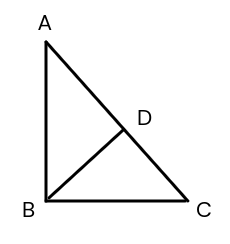
\includegraphics[width=3.5cm]{static/Screenshot from 2023-02-05 18-34-23.png}
    \caption{Inverse Pythagorean Theorem}
    \label{fig:galaxy}
\end{figure}
In the following figure, let, AB = c, BC = a, CA = b and BD = p, then, we have to prove the following statement:
\[\frac{1}{p^2} = \frac{1}{a^2} + \frac{1}{c^2}\]
We will prove this theorem by the help of area of triangles.
\[\Delta ABC = \frac{1}{2}.a.c = \frac{1}{2}.p.b\]
Squaring both sides, we obtain, 
\[(a.c)^2 = (p.b)^2\]
\[\frac{1}{a^2.c^2} = \frac{1}{p^2.b^2}\]
\[\frac{b^2}{a^2.c^2} = \frac{1}{p^2}\]
Using the pythagorean theorem, we obtain,
\[\frac{a^2 + c^2}{a^2.c^2} = \frac{1}{p^2}\]
Simplifying, we obtain, 
\[\frac{1}{a^2} + \frac{1}{c^2} = \frac{1}{p^2}\]
which is the requires statement. \\
Therefore, the inverse pythagorean theorem is proved with the help of area of triangles.
\end{document}
